\subsection{Interconnectivity} \label{subsec:interconnectivity}

Figure \ref{fig:interconnectivity} shows the robot combined with the litter collection system. As the litter collection system is fully waterproof, the chassis has a dedicated plate for mounting on its exterior, positioned at the front center of the robot. This arrangement allows the litter collection system to have a better view of potential litter when the robot is moving around the beach. The plate is also positioned at the bottom of the chassis height, reducing the necessary length of the litter collector to reach the ground and lowering the center of gravity. The area of the plate can easily be modified to accommodate various sizes of litter collection systems, depending on litter box dimensions. The spacing of the front legs and area on the lid for solar panels change accordingly to accommodate various litter boxes.

Another advantage of the plate design is that the fasteners used to hold the litter system do not go through the waterproofed chassis. The only connection to the inside of the chassis is for the electrical wires. A waterproof wire feed through seal is used for this purpose \cite{mcmaster-carr_plastic_2019}, as shown in Figure \ref{fig:chassis_topview}. Small holes were added in the corner of the mounting plate to evacuate any accumulated water.

The oDrive controllers for the litter collector are placed inside the chassis.

\begin{figure}
    \centering
    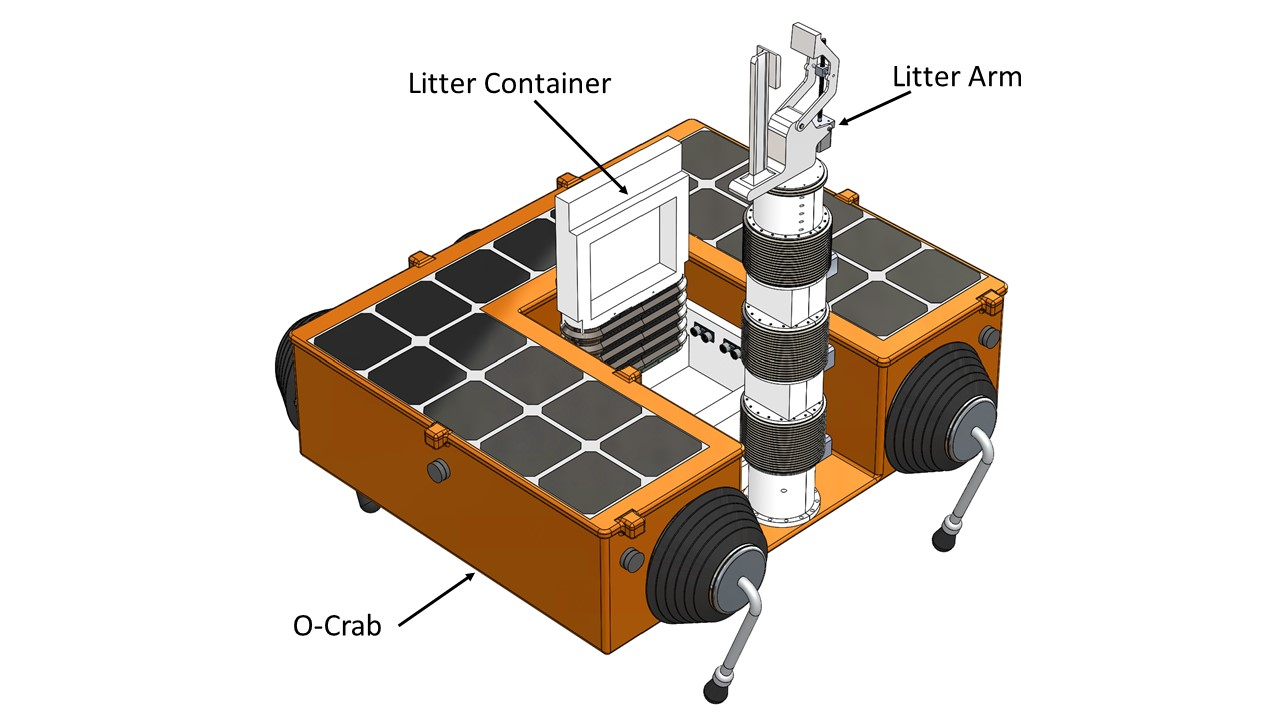
\includegraphics[width=\textwidth]{2_ProposedDesign/img/IsoWithArmA.jpg}
    \caption{Robot with litter collector system}
    \label{fig:interconnectivity}
\end{figure}
